\section{Introduction}

For the fourth laboratory assignment on our Circuit Theory and Electronics Fundamentals course, we had to improve, design and analyse an Audio Amplifier Circuit, which was especially interesting due to the presence of the BJT (Bipolar Junction Transistors), a new component we recently learned and were looking forward to understand experimentally the way it influences a circuit.

The circuit itself, as explained in our lectures, consisted of two different stages, the Gain Stage (which is designed with the objective of amplifying the voltage, in order to have the most possible gain) and the Output Stage (whose main goal is lowering the impedance of the gain stage, allowing the load to take almost full advantage of the gain). The full circuit can be seen in the picture below.

\begin{figure}[ht] \centering
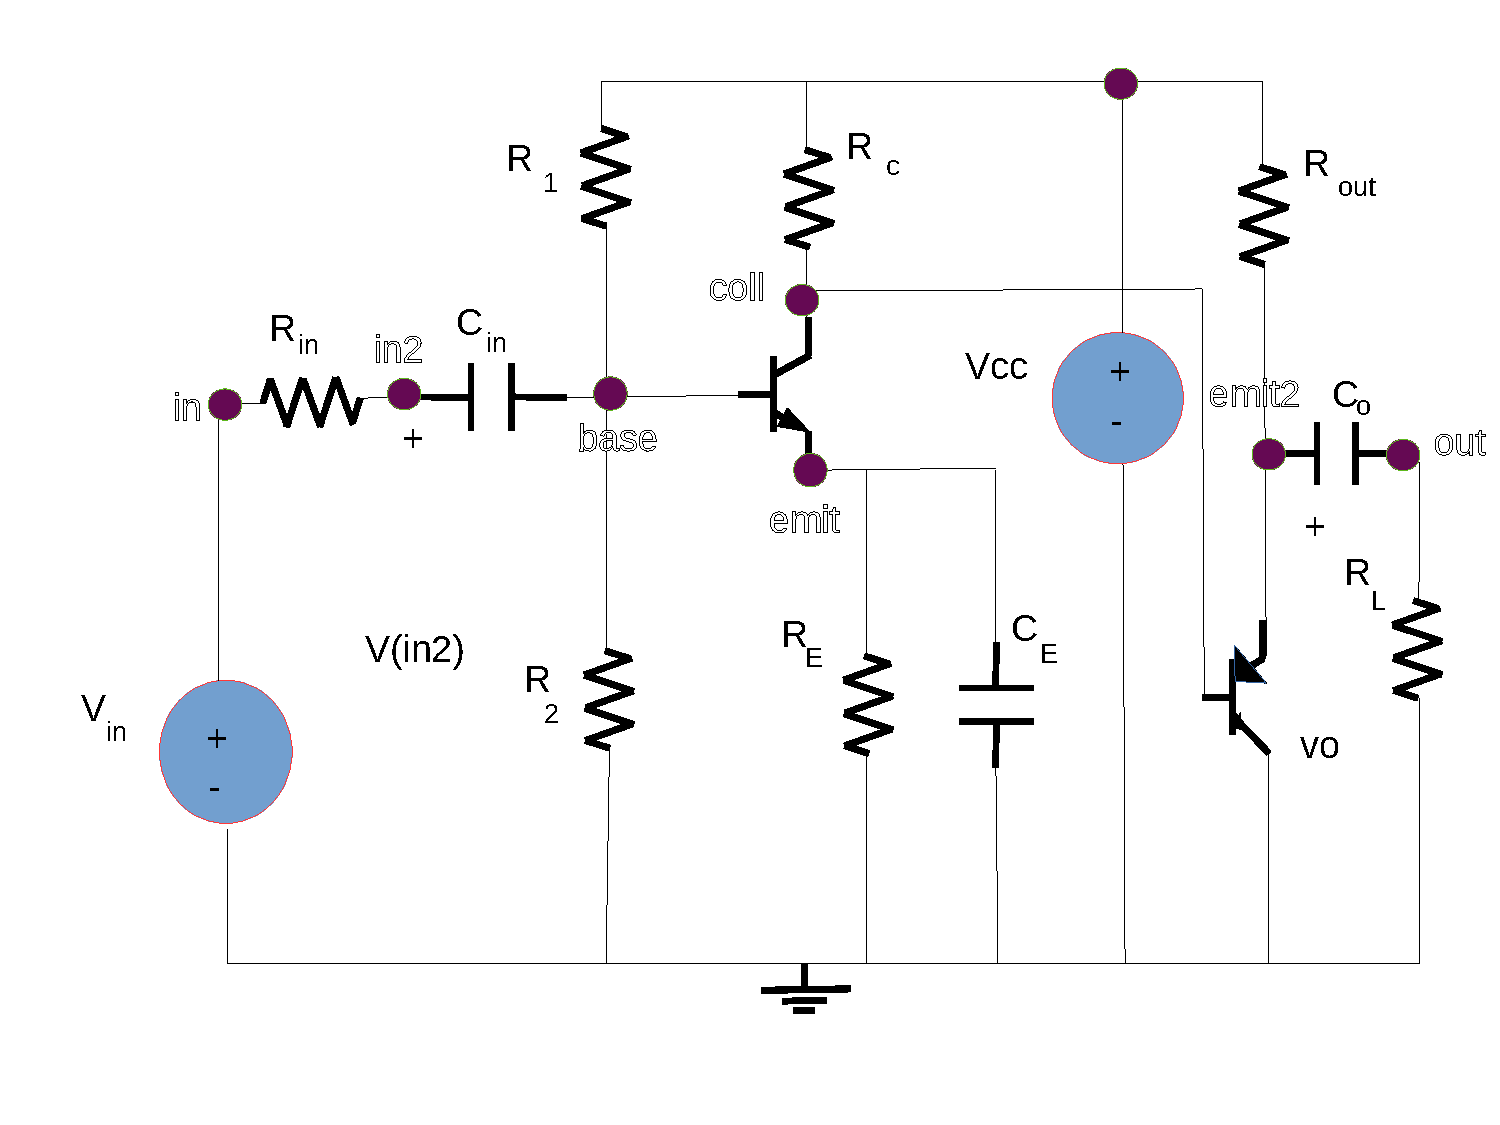
\includegraphics[width=0.7\linewidth]{lab4.pdf}
\caption{Circuit}
\label{fig:circ}
\end{figure}

\par
In this report, we will perform a comparison between our theoretical analysis and the simulation results, trying to explain any major discrepancies.


\clearpage

